\documentclass[10pt,a4paper]{article}
\usepackage[utf8]{inputenc} % para poder usar tildes en archivos UTF-8
\usepackage[spanish]{babel} % para que comandos como \today den el resultado en castellano
\usepackage{a4wide} % márgenes un poco más anchos que lo usual
\usepackage[conEntregas]{Sty/caratula}
\usepackage{Sty/mathtools}
\usepackage{Sty/float}
\usepackage[pdftex]{graphicx}
\usepackage{caption}
\usepackage{subcaption}
%\usepackage{Sty/algorithm2e}
\usepackage[ruled,vlined]{Sty/algorithm2e}
%Esto de abajo es para encabezado y pie de pagina
\usepackage{Sty/lastpage}
\usepackage{fancyhdr}
\usepackage{amsfonts}
\usepackage[noend]{algpseudocode}
\usepackage{enumerate} % AGREGO PARA PODER ENUMERAR LAS LINEAS DEL ALGORITMO
\usepackage{wrapfig}


\pagestyle{fancy}
%\fancyhf{} % clear all header and footer fields
%\fancyfoot[R]{\footnotesize Página \thepage\ de \lastpage\}

\cfoot{\thepage /\pageref{LastPage} }

%\newcommand\BlockIf[1]{\KwSty{If} \\ #1 \\ \KwSty{End If}}
\newcommand\BlockElseIf[1]{\KwSty{Else If} \\ #1 \\ \KwSty{End Else If}}
%\newcommand\BlockElse[1]{\KwSty{Else} \\ #1 \\ \KwSty{End Else}}
\newcommand{\Ode}[1]{\hfill O(#1)}
\newcommand{\WhileOde}[1]{\hfill \textit{en el peor caso el ciclo se ejecuta} #1 veces}
\newcommand{\IfOde}[1]{\hfill \textit{la complejidad de la sentencia del if es de} O(#1)}
\newcommand{\Tde}[1]{\hfill T(#1)}
\begin{document}



\fecha{\today}

\materia{Algoritmos y Estructuras de Datos III}
\titulo{Trabajo Práctico I}
%\grupo{Grupo Numero}

\integrante{Cadaval, Matias}{345/14}{matias.cadaval@gmail.com}
\integrante{Campos Paso, María Candelaria}{774/11}{cande.cp@gmail.com}
\integrante{Lew, Axel Ariel }{225/14}{axel.lew@hotmail.com}
\integrante{Noli Villar, Juan Ignacio}{174/14}{juaninv@outlook.com}

% Pongan cuantos integrantes quieran

\maketitle

\newpage
\tableofcontents		%compilar varias veces si no se actualiza el indice o el pie de pagina

\newpage
\section{Introducción}
En el presente trabajo resolveremos 3 problemas algorítmicos que nos fueron dados, respetando sus requerimientos de complejidad temporal, analizaremos empíricamente los tiempos de ejecución de sus implementaciones, mostraremos un pseudocódigo de los mismos, y las experimentaciones realizadas con sus debidos gráficos.




\section{Problema 1: \textbf{Telégrafo}}
\subsection{Idea general del problema}
Se ha decidido conectar telegráficamente todas las estaciones de un sistema férreo que recorre el país en abanico con origen en la capital (el kilómetro 0). Se nos ofrece cierta cantidad de kilometros de cable para conectar la ciudades de cada ramal. Al ser escaso el presupuesto, se busca lograr conectar la mayor cantidad de ciudades con los metros asignados, sin hacer cortes en el cable. \\

Se nos propone resolver cuántas ciudades se pueden conectar para cada ramal, con una complejidad de O(n), siendo n la cantidad de estaciones en cada ramal.\\

Para ello se nos brinda un archivo de entrada, el cual tiene para cada ramal dos líneas: la primera contiene un entero con los kilómetros de cable dedicados al ramal y la segunda los kilometrajes de las estaciones en el ramal sin considerar el 0. Luego de ejecutar nuestro algoritmo, la salida del mismo debe contener, para cada ramal de la entrada, una línea con la cantidad de ciudades conectables encontradas.\\

Un ejemplo de archivo de entrada puede ser, (extracto del archivo Tp1Ej1.in):\\
6 \\
6 8 12 15 \\
35 \\
8 14 20 40 45 54 60 67 74 89 99 \\
100 \\
35 87 141 163 183 252 288 314 356 387 \\
90 \\
6 8 16 19 28 32 37 45 52 60 69 78 82 \\

El mismo indica, en su primer línea que para el ramal 1 tenemos 6km de cable, y en su segunda línea que dicho ramal contiene (además de la capital, implícita, en el kilómetro 0) una estación en el kilómetro 6, otra en el 8, otra en el 12 y la última en el kilómetro 15. Luego para el ramal 2, tenemos 35 kilómetros de cable, y estaciones en los kilómetros: 8 14 20 40 45 54 60 67 74 89 y 99. Así sucesivamente para el resto de los ramales.\\

El archivo de salida luego de ejecutarse nuestro algoritmo deberá ser de la siguiente pinta, (extracto del archivo Tp1Ej1.out):\\
3 \\
6 \\
4 \\
14 \\

Este último archivo indica la cantidad de ciudades que se pueden conectar para cada ramal. En el caso del ramal 1, para el cual se tienen 6km de cable disponibles, y contiene ciudades en los kilómetros: 0 6 8 12 15 vemos que la solución debería ser que se pueden conectar como máximo 3 ciudades, a continuación explicaremos cómo se deduce esto.\\

Si conectamos la capital con la ciudad del kilómetro 6, al tener sólo 6km de cable, nuestra solución sería que pudimos conectar sólo 2 ciudades. Pero como debemos maximizar esta cantidad, podemos ver que si en vez de conectar a la capital con la primer estación del ramal, conectamos la ciudad del kilómetro 6, con su siguiente y con la del kilómetro 12, entonces como entre el kilómetro 6 y el 8 hay una diferencia de 2kms y entre el 8 y el 12 una diferencia de 4kms, vemos que la máxima cantidad de estaciones conectadas con 6km de cable para el ramal 1, es 3. La misma lógica se la aplica para los ramales restantes.\\


\subsection{Explicación y pseudocódigo}

int conectar(vector$<$int$>$ v , int longitud del cable) \{ \\
$~~~~~~~~~~~~$int resTemp $\leftarrow$ 1 \Ode{1}\\
$~~~~~~~~~~~~$int start $\leftarrow$ 0 \Ode{1}\\
$~~~~~~~~~~~~$int actual $\leftarrow$ 0 \Ode{1}\\
$~~~~~~~~~~~~$int aux $\leftarrow$ 0 \Ode{1}\\

$~~~~~~~~$\While{ (la longitud del cable sea $>$ 0 y v[actual] no sea el ultimo)} \{ \WhileOde{n} \\
$~~~~~~~~~~~~~~~$aux  $\leftarrow$ longitud del cable \Ode{1}\\
$~~~~~~~~~~~~~~~$\textbf{si} es el primer elemento del vector (el km 0) \IfOde{1}\\
$~~~~~~~~~~~~~~~~~~~~$a la longitud del cable le restamos el valor del segundo elemento. \Ode{1}\\
$~~~~~~~~~~~~~~~$\textbf{si no} es el kilómetro 0\\
$~~~~~~~~~~~~~~~~~~~~$a la longitud del cable le restamos la diferencia entre dicho elemento y su próximo.\Ode{1}\\

$~~~~~~~~$\}\\

$~~~~~~~~$\textbf{si} la longitud del cable sigue $>$ 0 \\
$~~~~~~~~~~~~~~~$incrementamos en 1 resTemp\Ode{1}\\
		
$~~~~~~~~$incrementamos en 1 actual, siempre.\Ode{1}\\

$~~~~~~~~$\textbf{si} resTemp sigue valiendo 1 \IfOde{1}\\
$~~~~~~~~~~~~~~~$ seteamos resTemp $\leftarrow$ 0; porque no se conectó ninguna ciudad. \Ode{1}\\

$~~~~~~~~$\textbf{si} nos pasamos y la longitud del cable $<$ 0  \IfOde{1} \\
$~~~~~~~~~~~~~~~$volvemos al valor anterior: la longitud del cable $\leftarrow$ 'aux' \Ode{1}\\

$~~~~~~~~$\While{la longitud del cable sea $>$ 0 y el elemento actual no sea el último)} \{ \WhileOde{n} \\
		int conectadas \\
$~~~~~~~~~~~~~~~$\textbf{si}(resTemp $\leftarrow$0)  \IfOde{1} \\
$~~~~~~~~~~~~~~~~~~~~$conectadas  $\leftarrow$ 0; \Ode{1}\\
$~~~~~~~~~~~~~~~~~~~~$start++; \Ode{1}\\
$~~~~~~~~~~~~~~~$\textbf{si no}
$~~~~~~~~~~~~~~~~~~~~$conectadas $\leftarrow$ resTemp - 1;\Ode{1}\\ 
$~~~~~~~~~~~~~~~~~~~~$longCable $\leftarrow$ longCable + (v[start+1]-v[start]);\Ode{1}\\
$~~~~~~~~~~~~~~~~~~~~$incrementamos start en 1;  \Ode{1}\\
$~~~~~~~~~~~~~~~~~~~~$\While{(longitud del cable $\geq$ 0 y v[actual] no es el último)} \{ \WhileOde{longitud del cable} \\
$~~~~~~~~~~~~~~~~~~~~~~~~~~~$aux $\leftarrow$ longCable; \Ode{1}\\
$~~~~~~~~~~~~~~~~~~~~~~~~~~~$a longitud del cable  le restamos (v[actual+1]- v[actual]); \Ode{1}\\
$~~~~~~~~~~~~~~~~~~~~~~~~~~~$incrementamos en 1 actual \Ode{1}\\
$~~~~~~~~~~~~~~~~~~~~~~~~~~~~~~~~$\textbf{si} (longitud del cable $\geq$ 0)  \IfOde{1}\\
$~~~~~~~~~~~~~~~~~~~~~~~~~~~~~~~~~~~~$incrementamos en 1 conectadas \Ode{1}\\
$~~~~~~~~~~~~~~~~~~~~~~~~~~~~~~~~$\textbf{si no} \\
$~~~~~~~~~~~~~~~~~~~~~~~~~~~~~~~~~~~~$longitud del cable $\leftarrow$ 'aux' \Ode{1}\\
$~~~~~~~~~~~~~~~~~~~~~$\} \\
$~~~~~~~~~~~~~~~~~~~~$\textbf{si} (conectadas $>$ resTemp)\IfOde{1}\\
$~~~~~~~~~~~~~~~~~~~~~~~~~~~~$resTemp $\leftarrow$ conectadas\Ode{1}\\
$~~~~~~~~$\}
$~~~~~~~~~~~~~~~~~~~~$\textbf{si} (resTemp es 1)\IfOde{1}\\
$~~~~~~~~~~~~~~~~~~~~~~~~~~~~$resTemp $\leftarrow$ 2;\Ode{1}\\
\}




\}\\

\subsection{Deducción de la cota de complejidad temporal}

Dedujimos que el algoritmo indica cuantas ciudades se pueden conectar, para cada ramal en O(n), siendo n la cantidad de estaciones en cada ramal, ya que..

\textbf{FALTA explicar porque dedujimos q es O(n)}

%Nuestro algoritmo, sin importar el archivo de entrada, recorre el vector de kilometrajes de ciudades de cada ramal \textbf{siempre}. Entonces decimos que el mejor caso es igual al peor caso,\textbf{ES CIERTO ESTO??}  por lo tanto

Vamos a mostrar la implementación de un test generado sin ninguna intencionalidad, pero antes explicaremos detalladamente como fue creado. \\

Implementamos una función que genera números random para el archivo que le vamos a pasar por entrada a nuestro algoritmo con los siguientes criterios:
\begin{itemize}
\item Elegimos en este ejemplo que el primer ramal iba a contar con una estación, el segundo con 101, el tercero con 201 y asi sumando de a 100.
\item Para el valor de la longitud de cable disponible de cada ramal, decidimos que sea un número random entre 1 y la cantidad de estaciones de cada ramal.
\item Para los kilometrajes de las estaciones tuvimos en cuenta, que estos debían estar ordenados de menor a mayor, sin contener el kilómetro 0. Para definir esto hacemos algo de la pinta:

ciudad = ciudad + (random.randrange(i+1)+1)

random.randrange(i+1) da un número random entre 0 e $i+1$, como inicialmente $i$ es 0 tuvimos que sumarle 1. A su vez a esto lo incrementamos en 1 porque un número random entre 0 e $i+1$ puede llegar a darnos 0, y no queremos que esto pase, ya que el kilómetro 0 no debe figurar en el archivo de entrada.

Por otro lado, al hacer $``$ciudad = ciudad + ...$"$ nos aseguramos que los kilometrajes esten en orden creciente.

\end{itemize}

Podemos ver el código de este test implementado en python acá:

--------------------------------------------------------------------------------\\
$~~~~~~$file = open('ejemploConNumerosRandom.in', 'w+')\\
$~~~~~~$file2 = open('ejemploTamCiudades.txt', 'w+')\\
$~~~~~~$for x in xrange(1,10000, 100):\\
$~~~~~~~~~~~~$i = 0\\
$~~~~~~~~~~~~$ciudad = 0\\
$~~~~~~~~~~~~$file.write(str(random.randrange(x)) + ' \textbackslash n')\\
$~~~~~~~~~~~~$file2.write(str(x) + ' \textbackslash n')\\
$~~~~~~~~~~~~$while i $<$ x:\\
$~~~~~~~~~~~~~~~~~~~~~~~~$ciudad = ciudad + (random.randrange(i+1)+1)\\
$~~~~~~~~~~~~~~~~~~~~~~~~$file.write(str(ciudad) + ' ')\\
$~~~~~~~~~~~~~~~~~~~~~~~~$i = i + 1\\
$~~~~~~~~~~~~$file.write(' \textbackslash n')\\
$~~~~~~$file2.close()\\

--------------------------------------------------------------------------------\\

Una vez que generamos el archivo del input con dicho test, ejecutamos nuestro algoritmo obteniendo el archivo de salida con la cantidad de ciudades conectadas para cada ramal, e imprimimos por pantalla el tiempo promedio en milisegundos que tardó nuestro algoritmo en calcular la máxima cantidad de estaciones conectadas de cada ramal. ¿Por qué el tiempo promedio? Bueno, al ejecutarlo un par de veces nos dimos cuenta que se obtenían valores parecidos pero no idénticos, entonces decidimos correr el algoritmo una cierta cantidad de iteraciones (en este caso 100), e ir acumulando los tiempos para luego dividir este acumulador por 100 y así obtener un valor promedio de los tiempos en los que se tarda en resolver el problema para cada ramal. \\

Con estos tiempos creamos el gráfico de la figura \ref{ej1-tiempo-vs-cant-ciudades-random} que mostramos a continuación, en el que hacemos una comparación con la gráfica de O(n) y observamos como nuestro algoritmo cumple dicha complejidad.


\begin{figure}[H]
\begin{center}

\minipage{0.8\textwidth}
  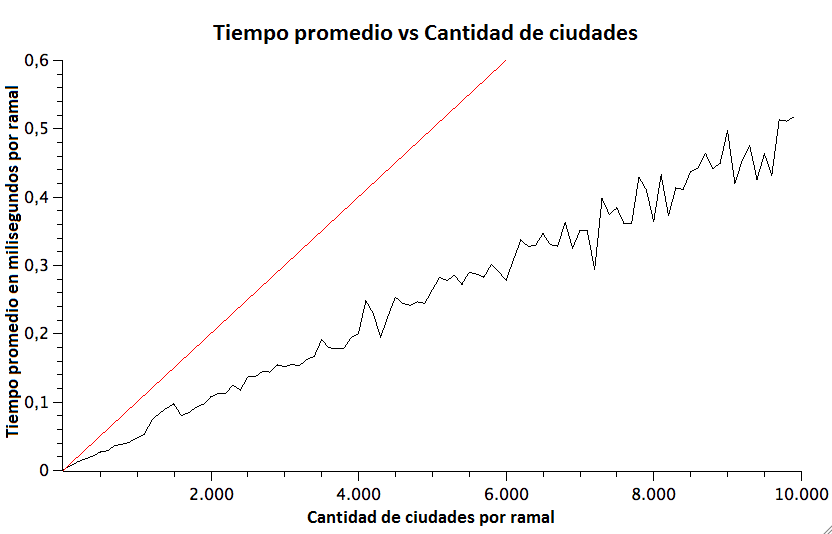
\includegraphics[width=\linewidth]{../graficos/ej1/1erEjTiempoPromedioVsO(n).png}
  \caption{{\small Comparación con O(n). Dado un archivo de entrada con longitud de cable y kilometrajes de estaciones random.}} \label{ej1-tiempo-vs-cant-ciudades-random}
\endminipage

\end{center}
\end{figure}
\subsection{Demostración formal}
\subsection{Experimentaciones}

\newpage
\section{Problema 2: \textbf{A Medias}}
\subsection{Idea general del problema}

\subsection{Pseudocódigo}



\subsection{Deducción de la cota de complejidad temporal}

\subsection{Demostración formal}
\subsection{Experimentaciones}

\newpage
\section{Problema 3: \textbf{Girls Scouts}}
\subsection{Idea general del problema}
El ejercicio nos propone diseñar un algoritmo para resolver el siguiente problema: dado un grupo de exploradoras, y el conjunto 
de amigas de cada una de ellas, organizar una ronda de manera tal que exista la menor distancia posible entre cada amistad, es 
decir, minimizar la suma de las distancias entre todos los pares de amigas. \\

La complejidad de la solución debe ser estrictamente menor que O($e^ea^2$), donde $e$ es la cantidad de exploradoras en cada grupo, y $a$ la cantidad de amistades. \\

Algunos ejemplos de posibles datos de entrada del problema son: \\

a bcde;b acde;c abde;d abc;e abc \\
a bcd;b ae;c ad;d ac;e b \\
a fb;b gc;d gc;f agh;e hd \\
x yz \\

Cada línea corresponde a un grupo de exploradoras; y se compone de una exploradora, seguida por una sucesion de amistades
separadas por ``;"$ $. Por ejemplo, en la primer línea, el grupo de exploradoras esta compuesto por ``a"$ $ cuyas amigas son [bcde],
``b"$ $ con [acde], ``c"$ $ con [abde] y por último ``d"$ $ y ``e"$ $ con  [abc]. Asumimos que las amistades son simétricas, es decir, si ``a"$ $ es
amiga de ``b"$ $, entonces ``b"$ $ es amiga de ``a"$ $. Por lo tanto, aunque ocurra que ``x"$ $ este en el conjunto de amigas de ``y"$ $, pero ``y"$ $ no este en el de ``x"$ $, debemos interpretarlo como que cada una esta en el grupo de amigas de la otra.  \\

Las salidas que corresponden a los ejemplos recien dados son las siguientes (mismo orden): \\
2 abdce \\
2 abecd \\
3 abgcdehf \\
1 xyz \\

La sucesión de caracteres representa la solución del problema, es decir, la ronda en la que exista la menor distancia posible entre cada amistad. El número que está delante, es la máxima distancia que hay entre dos amigas en la ronda solución. Si es que existe mas de una ronda óptima, se debe dar la que esté primera alfabéticamente. 

\subsection{Explicación y pseudocódigo}
Para resolver el problema diseñamos un algoritmo que consiste en, dado un grupo de exploradoras, generar todas las rondas 
posibles, e ir almacenando aquella que hasta el momento es la ``mejor"$ $ entre las ya calculadas (con ``mejor"$ $ nos referimos a aquella que minimiza la suma de las distancias entre amigas).\\

Para armar las permutaciones utilizamos la funcion $next$\_$permutation$, perteneciente a la librería standard de c++. Mediante 
esta funcion vamos generando todas las rondas posibles en orden alfabético. Entonces, a medida que vamos armando las 
distintas rondas posibles, calculamos la suma de distancias y luego la comparamos con la suma de la que tenemos almacenada. Si 
la suma de la nueva ronda es menor entonces nos guardamos la nueva, pues es ``mejor"$ $ que la que teníamos. Caso contrario, 
pasamos a calcular la siguiente ronda, pues si la suma es mayor esa ronda no nos interesa, y si es igual tampoco, porque como
las rondas se van calculando en orden alfabetico, entonces la que ya tenemos guardada va a estar primera teniendo en cuenta
dicho orden. \\

El algoritmo termina una vez que se hayan calculado todas las rondas posibles. La última ronda que quedó guardada va a ser nuestra solución. Por otra parte, la máxima distancia entre dos amigas de la ronda, se calcula en simultáneo con la suma de las distancias, y siempre la almacenamos junto con la ``mejor"$ $ ronda durante todo el algoritmo. \\

Para entender mejor la idea dejamos el algoritmo en pseudocódigo:\\   
--------------------------------------------------------------------------------------------------------------\\
mejorRonda (dado un conjunto de exploradoras (exp) y sus amistades) \\
$~~~~~~~~$crear int sumaMinima \\
$~~~~~~~~$crear int maxDist \\
$~~~~~~~~$crear Ronda rondaOptima  \\
$~~~~~~~~$ordenar alfabeticamente exp \\
$~~~~~~~~$rondaOptima $\leftarrow$ exp \\
$~~~~~~~~$sumaMinima $\leftarrow$ calcular suma de distancias de rondaOptima  \\
$~~~~~~~~$maxDist $\leftarrow$ calcular maxima distancia entre 2 amigas en rondaOptima \\
$~~~~~~~~$\textbf{mientras} (hay nueva permutacion de exp) \{ \\
$~~~~~~~~~~~~$crear int nuevaSuma $\leftarrow$ calcular suma de distancias de exp  \\
$~~~~~~~~~~~~$crear int nuevaDist $\leftarrow$ calcular maxima distancia entre 2 amigas en exp  \\
$~~~~~~~~~~~~$\textbf{si} (nuevaSuma $<$ sumaMinima) \{ \\
$~~~~~~~~~~~~~~~~$ sumaMinima $\leftarrow$ nuevaSuma \\
$~~~~~~~~~~~~~~~~$ maxDist $\leftarrow$ nuevaDist \\
$~~~~~~~~~~~~~~~~$ rondaOptima $\leftarrow$ exp \\
$~~~~~~~~~~~~$\} \\
$~~~~~~~~$ \} \\
$~~~~~~~~$ exp $\leftarrow$ rondaOptima\\
$~~~~~~~~$ devolver maxDist\\
--------------------------------------------------------------------------------------------------------------\\ \\
El calculo de la suma de las distancias lo hacemos mediante un algoritmo iterativo que, lo que hace, es recorrer el vector
(que representa a la ronda), y para cada exploradora calcula cuál es la ditancia entre ella y cada una de sus amigas (mediante 
otro ciclo interno). Se repite el procedimiento hasta que el vector se recorre completamente, y así obtenemos la suma de las distancias.  


\subsection{Deducción de la cota de complejidad temporal}

Para la resolución de este ejercicio construimos la clase Ronda en c++. La ronda se representa, en la parte privada de la clase,
mediante un vector$<$char$>$, donde los char representan a las exploradoras y cómo están ubicadas en la ronda. También posee un 
diccionario(utilizamos $<$map$>$ de la STL de c++), donde están asociadas las exploradoras a sus respectivos grupos de amigas. \\
La clase cuenta con el constructor por defecto (ronda vacia) y otro constructor que recibe como parámetros un vector$<$char$>$ y un
vector$<$vector$<$char$>>$; donde el primero representa el conjunto de exploradoras, y el segundo las amigas de cada una (asociadas
por el orden de los vectores). Como el enunciado del ejercicio permite que mismos grupos de exploradoras sean escritos de distintas 
formas (por ejemplo a bc;b ac;c ab también se puede escribir como a b;b c;c ab), construimos la función $completarAmigas$ que se 
encarga de verficar que ninguna amistad esté ausente en la lista de una exploradora, y que estén presentes la totalidad de las 
exploradoras, cada una con su grupo de amigas. Esta función la utilizamos en el constructor, de manera que se almacene en la parte 
privada toda la información completa. \\
A continuación analizamos paso a paso la complejidad temporal de las funciones que implementamos. Para ello, tener en cuenta que 
$e$ representa la cantidad de exploradoras de cada grupo, y $a$, la cantidad de amistades. \\
La complejidad de $completarAmigas$ es O($e^3$) en el peor caso; y el algoritmo consiste en los siguientes pasos (recibe los mismos parámetros de entrada que el constructor): \\
\begin{itemize}
\item Recorrer el vector$<$char$>$ que contiene i exploradoras. \\
Costo: O($e$) pues como maximo  e = i. 
\item Por cada una de las exploradoras recorrer su grupo de amigas. \\
Costo: O($e$) pues como maximo son e - 1 amigas.
\item Por cada amiga, verificar si está presente en el vector de exploradoras y en caso positivo (si no está presente se agrega, que 
toma O(1)), verificar si la exploradora i está presente en el grupo de dicha amiga(si no está presente se agrega, que 
toma O(1)).  \\
Costo: O($e$) pues son dos busquedas lineales con costo O($e$) en el peor caso cada una.
\end{itemize}
Finalmente la ecuación de la complejidad del algoritmo es O($e$) x O($e$) x O($e$) = O($e^3$). \\
Otra operación pública de nuestra clase es $sumaDistancias$, que devuelve una dupla de enteros, donde la primer componente 
representa la suma de las distancias entre las exploradoras que son amigas, y la segunda, la mayor distancia entre dos amigas en 
la ronda. A continuación analizamos la complejidad de $sumaDistancias$: 
\begin{itemize}
\item Recorrer el vector$<$char$>$ que contiene a las exploradoras. \\
Costo: O($e$) pues siempre las rondas tienen e exploradoras.
\item Por cada exploradora buscar su grupo de amigas en el diccionario y copiarlo a un vector auxiliar. \\
Costo: O($e$) pues buscar en el diccionario es O(log($e$))(extraido de cppreference.com) y copiarlo es O($e$).
\item Por cada amiga buscamos su posición en la ronda y calculamos la distancia entre ella y la exploradora a la que le corresponde el vector de amigas que estamos recorriendo. \\
Costo: O($e$) pues es buscar su posicion linealmente sobre e elementos, y el cálculo es O(1).
\end{itemize}
Finalmente la ecuación de la complejidad del algoritmo es O($e$) x O($e$) x O($e$) = O($e^3$). \\
\\
Otras operaciones que implementamos en la clase Ronda son: 
\begin{itemize}
\item $cambiarOrden$; que cambia las posiciones de las exploradoras en la ronda (lo hace en orden alfabético). Utilizamos la función 
$next$\_$permutation$ de la STL de c++, por lo que la complejidad es O($e$) en el peor caso(extraido de cppreference.com). 
\item $ordenAlfabetico$; que ordena la ronda alfabéticamente. Para ello usamos la función $sort$ de la STL, con complejidad
O($e$ log($e$)) (extraido de cppreference.com).
\end{itemize}
Ahora analicemos la complejidad de la principal operación del ejercicio, a la cual llamamos $mejorRonda$, que modifica la Ronda de manera
tal que minimice la suma de las distancias entre amigas, y devuelve la maxima distancia entre dos amigas en la ronda solución: 
\begin{itemize}
\item Ordenamos la ronda mediante $ordenAlfabetico$. \\
Costo: O($e$ log($e$))
\item Hacemos $sumaDistancias$ sobre la ronda ordenada, y guardamos los valores en una dupla de enteros.\\
Costo: O($e^3$)
\item Copiamos la ronda actual en una nueva variable. \\
Costo: O($e$)
\item Hacemos un ciclo que finaliza cuando hayamos generado todas las permutaciones posibles de la ronda. \\
Costo: O($e!$) (cantidad de iteraciones)
\item Por cada iteracion del ciclo realizamos lo siguiente (en el peor de los casos):\\
-$cambiarOrden$ (toma O($e$)) \\
-$sumaDistancias$ (toma O($e^3$)) \\
-Copiamos una ronda (toma O($e$))
\item Copiamos la mejor ronda en la parte privada de la Ronda. \\
Costo: O($e$)
\item Copiamos un entero a una nueva variable. \\
Costo: O(1)
\end{itemize}
Entonces, la complejidad de la función es:\\
O($e$ log($e$)) + O($e^3$) + O($e$) + O($e!$) x \big( O($e$) + O($e^3$) + O($e$) \big) + O($e$) + O(1) 









\subsection{Demostración formal}
El procedimiento que utilizamos resuelve el problema porque, dada una ronda, al combinar las exploradoras de todas las maneras 
posibles

\subsection{Experimentaciones}

%\subsection{Idea general del problema}
%\newpage
%\subsection{Explicación y pseudocódigo}
%\newpage
%\subsection{Justificación}
%\newpage
%\subsection{Deducción de la cota de complejidad temporal}
%\newpage
%\subsection{Análisis experimental de la complejidad}


\newpage
\section{Código}
%\subsection{Conclusión}

En este trabajo realizamos 3 algoritmos distintos que resuelven los ejercicios que nos presentaron, también medimos sus complejidades y las analizamos generando tests de mejor y peor caso, y de casos random. Ilustramos estos resultados con gráficos. Para realizarlos, siempre tomamos el tiempo promedio de 100 ejecuciones del algoritmo, para no considerar los tiempos de lectura/escritura. Además de explicarlos con ejemplos y pseudocódigos, analizamos la correctitud de estos algoritmos.


%\newpage
%\section{Bibligraf\'ia y recursos}
%\input{bibliografia}

\end{document}
